\section{Results}

\begin{frame}{result}
    \begin{table}[htb!]
        \centering
        \setlength{\tabcolsep}{1.5em}
        \renewcommand{\arraystretch}{1.5}
        \resizebox{0.9\textwidth}{!}{
        \begin{tabular}{l|ccc}
                               & counting              & shape                 & LEP \\
        \hline                                                                 
        w/o LU &&& \\
        \hline
        $\BWe$      & $(11.15 \pm 0.27) \%$ & $(10.77 \pm 0.1) \%$  & $(10.71 \pm 0.16)$ \% \\
        $\BWm$      & $(11.13 \pm 0.22) \%$ & $(10.91 \pm 0.08) \%$ & $(10.63 \pm 0.15)$ \% \\
        $\BWt$      & $(10.63 \pm 0.65) \%$ & $(10.89 \pm 0.21) \%$ & $(11.38 \pm 0.21)$ \% \\
        $\BWh$      & $(67.08 \pm 0.72) \%$ & $(67.42 \pm 0.28) \%$ & $(-- \pm --)$ \% \\
        \hline
        w/ LU &&& \\
        \hline
        $\BWl$      & $(-- \pm --)\%$       & $(10.87 \pm 0.07)\%$  & $(10.86 \pm 0.09)\%$  \\
        $\BWh$      & $(-- \pm --)\%$       & $(67.38 \pm 0.22)\%$  & $(67.41 \pm 0.27)\%$  \\
        \end{tabular}
        }
    \end{table}


    \begin{table}[htb!]
        \centering
        \renewcommand{\arraystretch}{1.5}
        \resizebox{0.9\textwidth}{!}{
        \begin{tabular}{ccc}
            counting              & shape                 & LEP \\
          $\begin{bmatrix} 1 &+0.576 &-0.060 \\  +0.576 &1 &-0.265 \\ -0.265 &+0.714 &1 \end{bmatrix}$  
        & $\begin{bmatrix} 1 &+0.439 &+0.138 \\  +0.439 &1 &+0.190 \\ +0.138 &+0.190 &1 \end{bmatrix}$ 
        & $\begin{bmatrix} 1 &+0.136 &-0.201 \\  +0.136 &1 &-0.122 \\ -0.201 &-0.122 &1 \end{bmatrix}$ \\
        \end{tabular}}
    \end{table}
\end{frame}

\begin{frame}{result}
    \begin{center}
    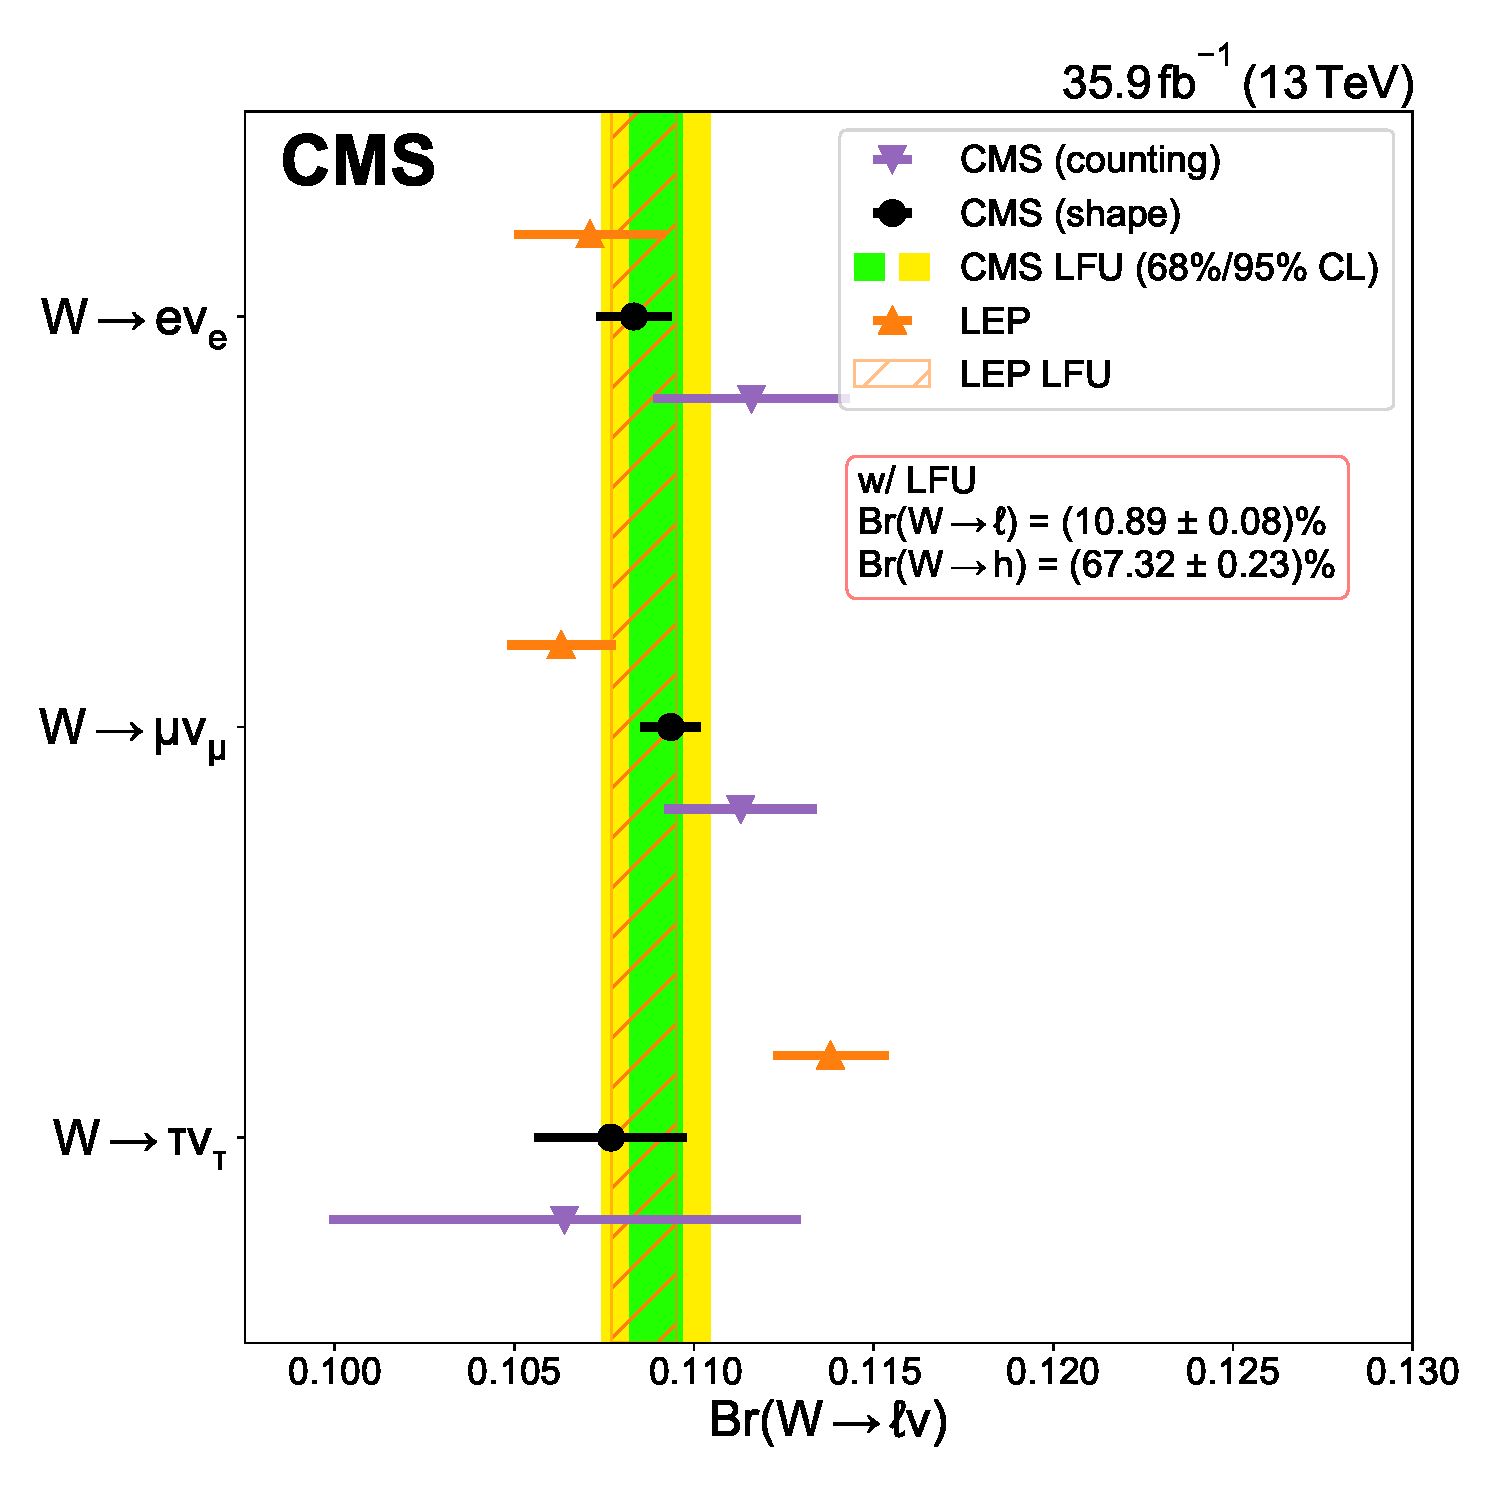
\includegraphics[width=0.6\textwidth]{chapters/Analysis/sectionResult/figures/unblinded_summary_plot.pdf}
    \end{center}
\end{frame}

% \begin{figure}[htb!]
%     \begin{center}
%     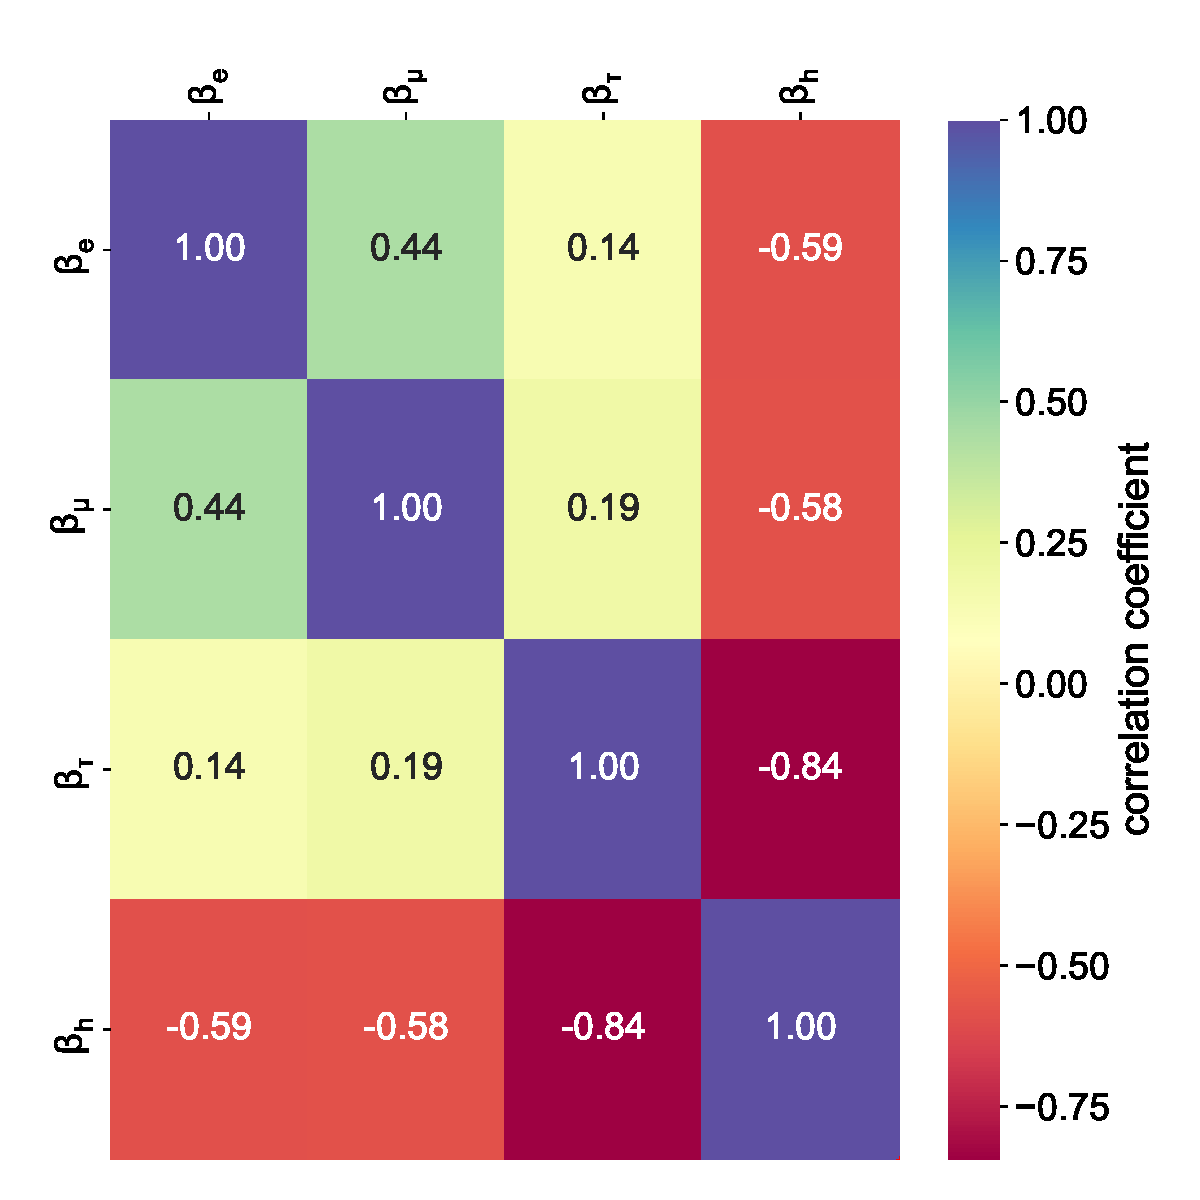
\includegraphics[width=0.5\textwidth]{chapters/Analysis/sectionResult/figures/correlation_matrix_POI_unblinded.pdf}
%     \caption{Correlation matrix between each branching fraction component.}
%     \label{fig:analysis:result:correlation_matrix_POI}
%     \end{center}
% \end{figure}

\begin{frame}{result}
    \begin{center}
    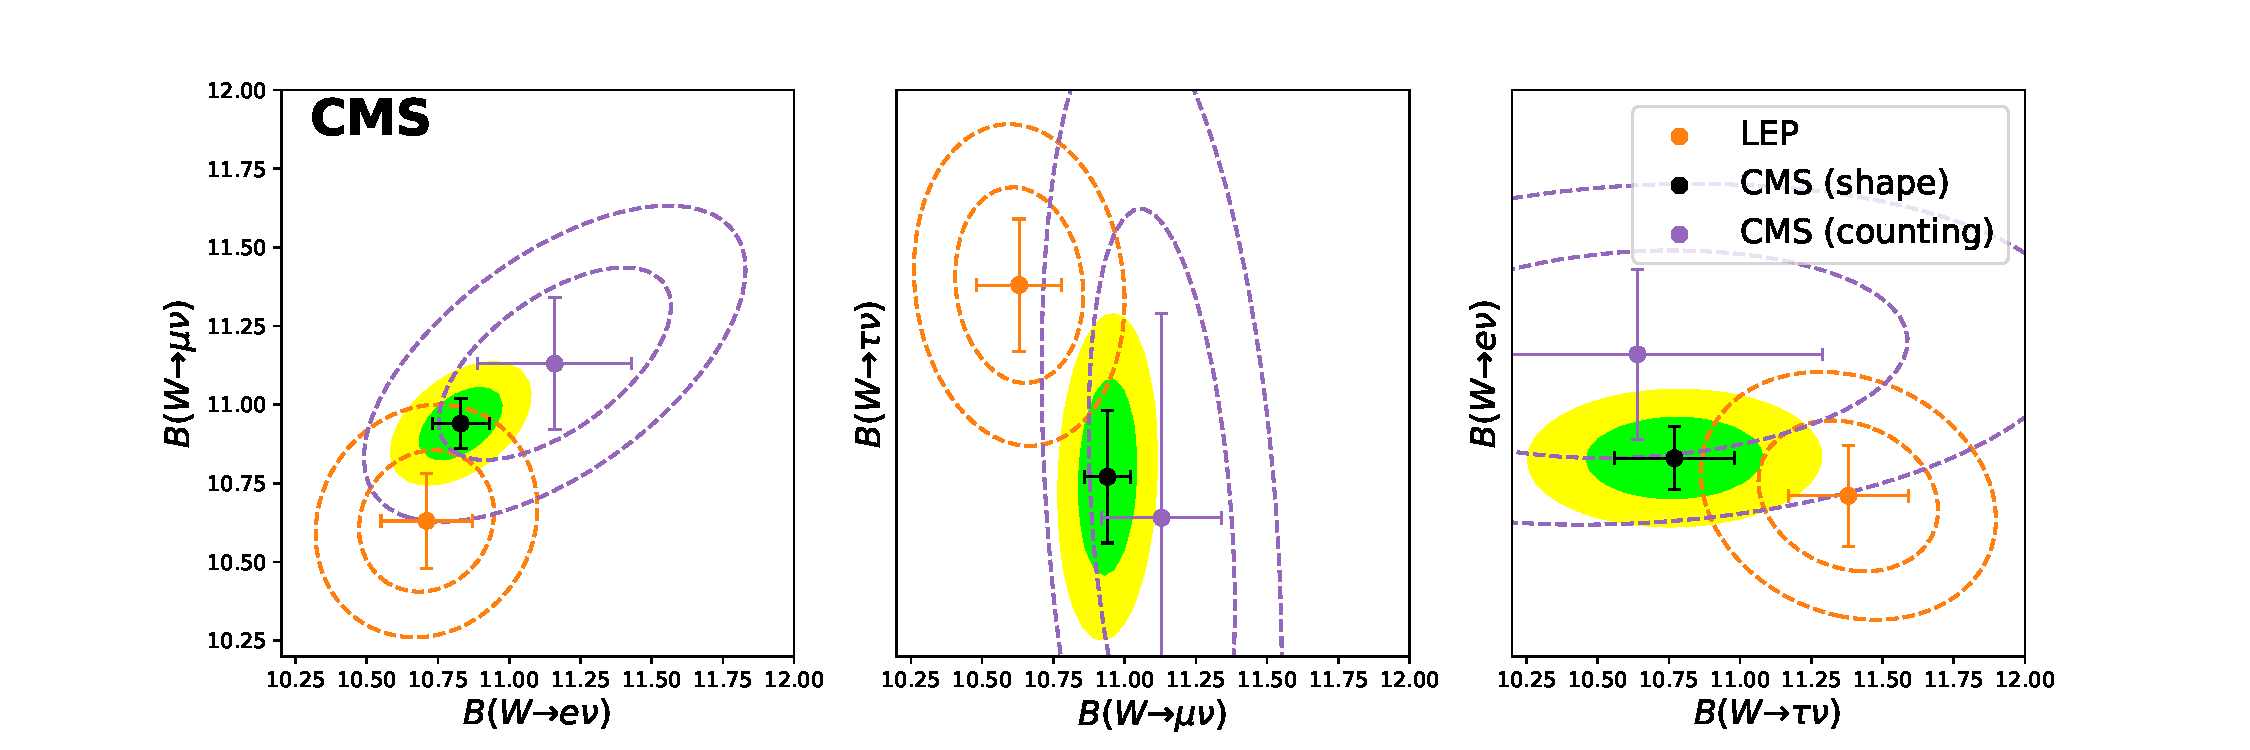
\includegraphics[width=0.99\textwidth]{chapters/Analysis/sectionResult/figures/result_contours_2d.pdf}
    \end{center}
\end{frame}


\begin{frame}{result}
    \begin{equation}
        f(r_{\PGt/\Pe}, r_{\PGt/\PGm}) = \int_{-\infty}^{\infty}
        \left| \beta_{\PGt}\right|g(r_{\PGt/\Pe}\beta_{\PGt}, r_{\PGt/\PGm}\beta_{\PGt}, \beta_{\PGt})
        d\beta_{\PGt}
    \end{equation}
    
    \begin{table}[htb!]
        \centering
        \setlength{\tabcolsep}{0.5em}
        \renewcommand{\arraystretch}{2}
        \resizebox{0.9\textwidth}{!}{
        \begin{tabular}{c|ccc}
                                & CMS               & LEP               & ATLAS              \\
        \hline                                                                 
        $\BWm / \BWe$           & $1.013 \pm 0.009$ & $0.993 \pm 0.019$ & --                 \\
        $\BWt / \BWe$           & $1.011 \pm 0.020$ & $1.063 \pm 0.027$ & --                 \\
        $\BWt / \BWm$           & $0.998 \pm 0.019$ & $1.070 \pm 0.026$ & $0.992 \pm 0.013$  \\
        $2 \BWt /(\BWe + \BWm)$ & $1.002 \pm 0.019$ & $1.066 \pm 0.025$ & --                 \\
        \end{tabular}}
    \end{table}
\end{frame}



\begin{frame}{result}
    \begin{figure}[htb!]
        \begin{center}
        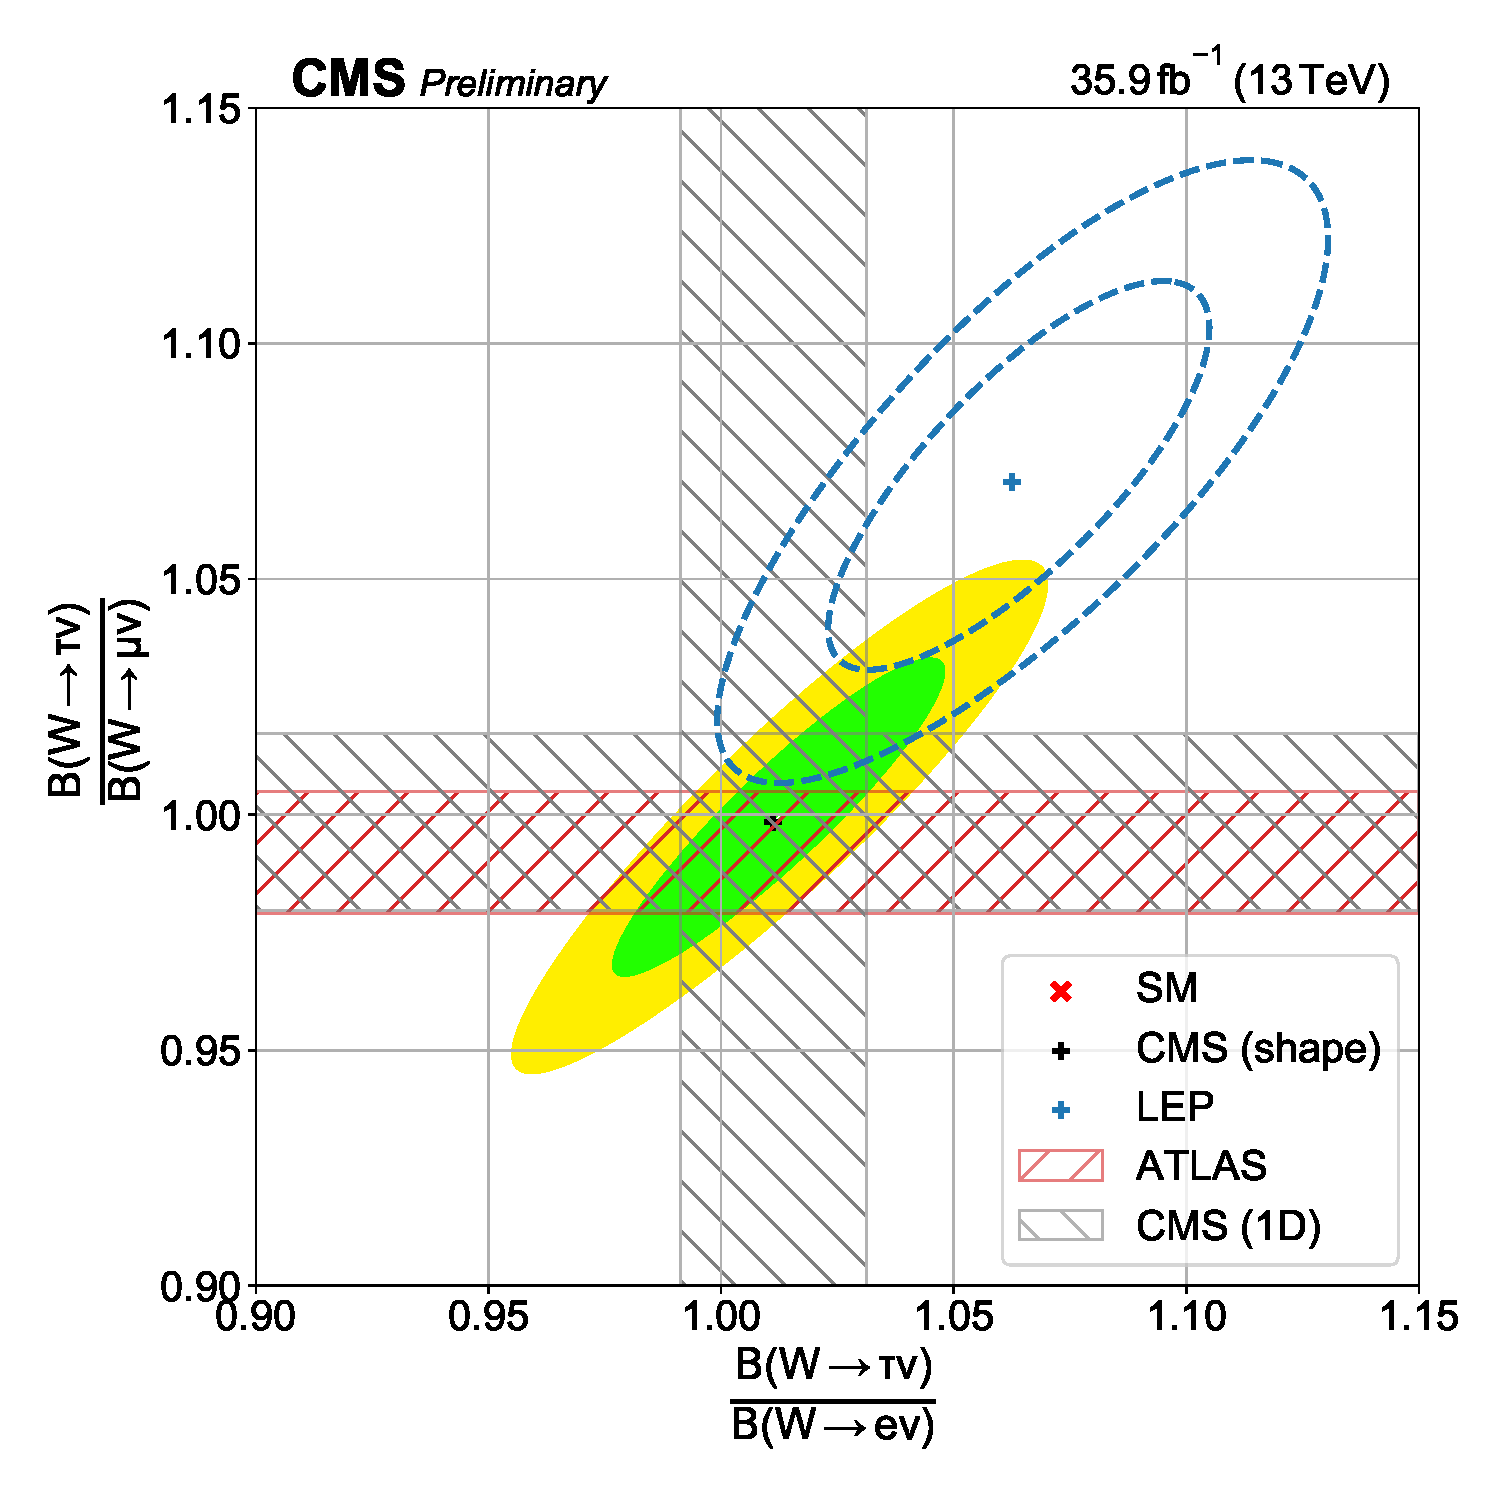
\includegraphics[width=0.7\textwidth]{chapters/Analysis/sectionResult/figures/result_contours_2d_ratio.pdf}
        \caption{Two dimensional distributions of the ratios $\BWt/\BWe$ vs $\BWt/\BWm$ 
        with comparisons of the CMS result to LEP and ATLAS measurements.}
        \label{fig:analysis:result:ratios_2D}
        \end{center}
    \end{figure}
\end{frame}



\begin{frame}{result}

\begin{equation}
    R^\PW_{\mathrm{h}/\ell} = \frac{\BWh }{1- \BWh} = \bigg( 1 + \frac{\alpS(m_\PW)}{\pi}\bigg) \sumCKM,
\end{equation}

\noindent where $\alpS(m_\PW)$ is the strong coupling constant at the $\PW$ pole. 


    \begin{table}[!h]
        \setlength{\tabcolsep}{0.5em}
        \renewcommand{\arraystretch}{2.5}
        \centering
        \resizebox{0.9\textwidth}{!}{
        \begin{tabular}{ccc|ccc}
            Assumption &  &  Quantity & CMS & LEP & CMS+LEP\\
            \hline
                                                                &                   & $R^\PW_{\mathrm{h}/\ell}$ & $2.060\pm0.021$ & $2.068\pm0.025$ & $2.063\pm0.016$ \\ \hline
            CKM Unitarity: $\sumCKM = 2$                        & $\Longrightarrow$ & $\alpS(m_\PW)$            & $0.094\pm0.033$ & $0.108\pm0.040$ & $0.099\pm0.026$ \\ \hline
            PDG~\cite{pdg2020} $\alpS(m_\PW) = 1.1200\pm0.010$  & $\Longrightarrow$ & \sumCKM                   & $1.985\pm0.021$ & $1.997\pm0.025$ & $1.992\pm0.016$ \\ \hline
            $\begin{matrix} 
                \text{PDG~\cite{pdg2020}: } \alpS(m_\PW) = 1.1200\pm0.010 \\ 
                \text{PDG~\cite{pdg2020}: } \sum_{\substack{ud,us,ub\\cd,cb}} |V_{ij}|^2 =1.0490(18) 
            \end{matrix} $ 
                                                                & $\Longrightarrow$ & \absVcs                   & $0.969\pm0.011$ & $0.974\pm0.013$ & $0.971\pm0.008$ \\ 
        \end{tabular}
        }
    \end{table}
\end{frame}

  
\begin{frame}{result}
    \begin{figure}[!h]
        \centering
        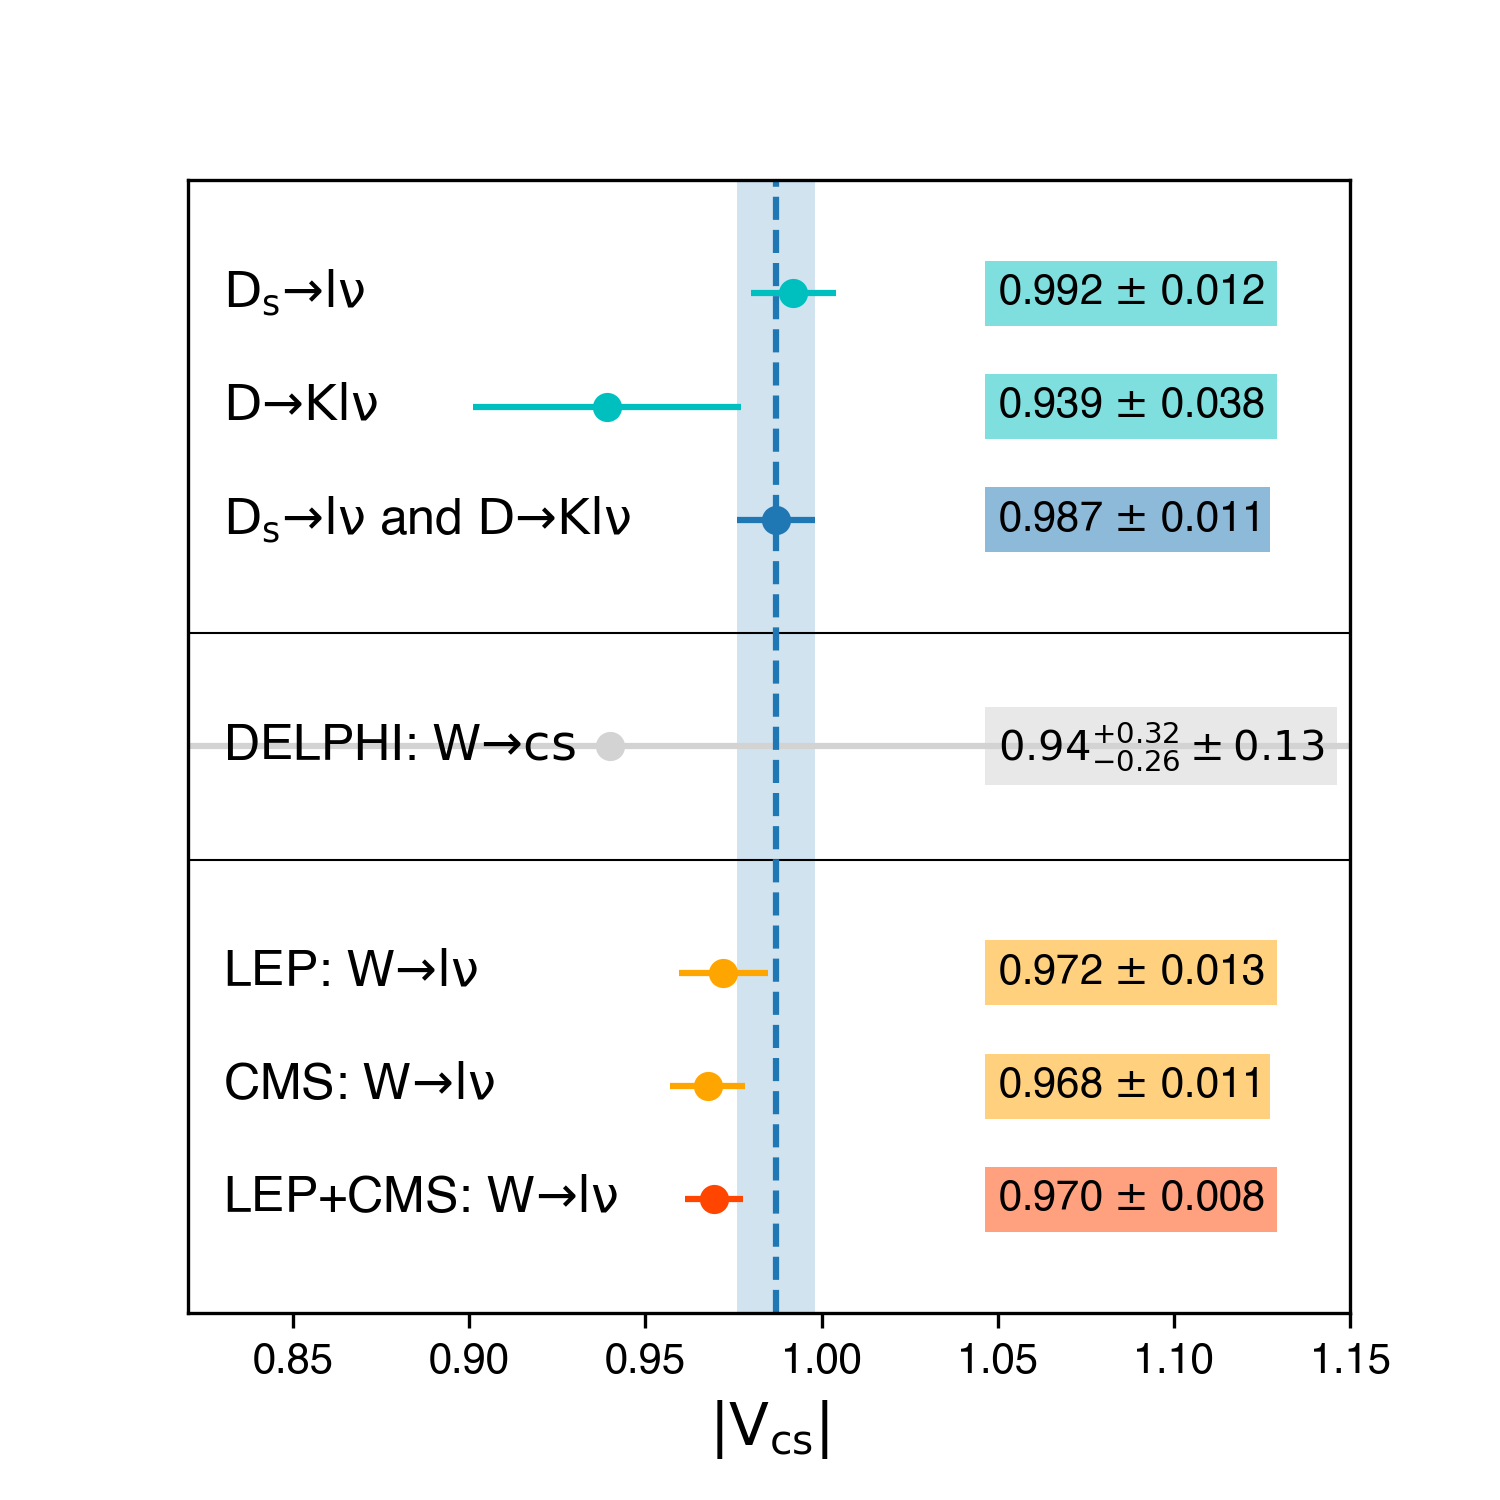
\includegraphics[width=0.6\textwidth]{chapters/Introduction/sectionRelatedWorks/figures/vcs.png}
        \caption{The \absVcs derived from the \BWl measurement by CMS, LEP and CMS+LEP, in comparison with the direct measurements~\cite{pdg2020}.}
        \label{fig:analysis:result:vcs}
    \end{figure}
\end{frame}


